\begin{figure}
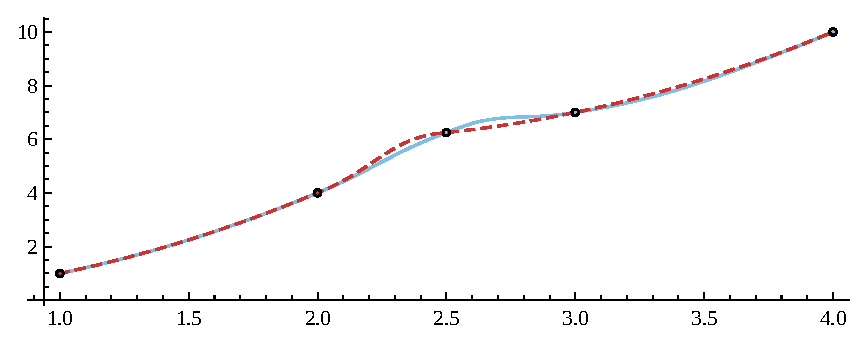
\includegraphics[width=4in]{vis/1-sensitivity.eps}
\caption{ % \everymath={\scriptstyle}  % \narrower\noindent\rmVIII Fig.\ 1.
  A demonstration of the quadratic facet model's sensitivity to small
  data perturbations. This example is composed of two quadratic
  functions $f_1(x) = x^2$ over points $\{1$, $2$, $5/2\}$, and
  $f_2(x) = (x-2)^2 + 6$ over points $\{5/2$, $3$, $4\}$. Notably,
  $f_1(5/2) = f_2(5/2)$ and $f_1$, $f_2$ have equal second
  derivatives. Given the exact five data points seen above, the
  quadratic facet model produces the slope seen in the solid blue line
  at $x = 5/2$. However, by subtracting the value of $f_3$ $=
  \epsilon(x-2)^2$ from points at $x = 3$, 4, where $\epsilon$ is the
  machine precision ($2^{-52}$ for an IEEE 64-bit real), the quadratic
  facet model produces the slope seen in the dashed red line at $x =
  5/2$. This is the nature of a facet model and a side effect of
  associating data with local facets.}
\end{figure}


\section{COMPLEXITY AND SENSITIVITY}

Algorithms 1 and 4 have $\mathcal{O}(n)$ runtime for $n$ data
points. Algorithm 2 has a fixed cost $\mathcal{O}(1)$. Given a fixed
schedule for shrinking derivative values, Algorithm 3 has a
$\mathcal{O}(n)$ runtime for $n$ data points. In execution, the
majority of the time, still $\mathcal{O}(n)$, is spent solving the banded
linear system of equations for the B-spline coefficients. Thus for $n$
data points, the overall execution time is $\mathcal{O}(n)$.

The quadratic facet model produces a unique sensitivity to input
perturbation, as small changes in input may cause different quadratic
facets to be associated with a breakpoint, and thus different initial
derivative estimates can be produced. This phenomenon is depicted in
Figure 1. Despite this sensitivity, the quadratic facet model is still
preferred because it exactly captures local linear and quadratic
behavior while empirically producing final approximations with less
wiggle (local $L^2$ norm of the second derivative) than other methods. A
weighted harmonic mean estimate of first derivatives may be more
accurate when the underlying function changes at a rate greater than a
quadratic, but that method increases the second derivative sensitivity
to small perturbations in data and empirically results in quintic
splines with greater wiggle.

The binary search for a point on the monotone boundary in $(\tau_1$,
$\alpha$, $\beta$, $\gamma)$ space is performed because it results in
monotone quintic spline interpolants with derivative values that are
absolutely nearer to initial estimates than a search that strictly
shrinks derivative values. Given that the initial derivative estimates
have desirable properties (capture low-order phenomena and are low
wiggle), this search results in an approximation that is both monotone
and has derivative values similar to the initial estimates.

The binary search procedure provably converges on the boundary of the
region of monotonicity precisely defined by Ulrich and Watson
\cite{ulrich1994positivity} through the application of a Boolean
function that is guaranteed to be true at one end of an
interval. Since a local quadratic interpolant is applied for initial
function derivative estimates, the approximation order of the
resulting fit is $O(h^3)$ (as for any second order approximation), but
it should be noted that asymptotic approximation order is rarely of
importance when considering the scattered sparse data that $C^2$
approximations like {\tt MQSI} provide. Were exact evaluations
provided, higher order methods always win (all other things being
equal) as the data density increases. For sparse data, what
constitutes a better fit is either subjective or dependent on the
problem.
